\documentclass[10pt,journal,compsoc]{IEEEtran}
\usepackage{grffile}
\usepackage[dvips]{graphicx}
\usepackage[cmex10]{amsmath}

\hyphenation{}

\begin{document}

\title{La eterna espera}


\author{Lucila Stancato,~\IEEEmembership{I.T.B.A,}
		Dami\'an Modernell,~\IEEEmembership{I.T.B.A,}
		Juan Brasca,~\IEEEmembership{I.T.B.A,}
		Conrado Negro,~\IEEEmembership{I.T.B.A}%
}

\IEEEcompsoctitleabstractindextext{%
\begin{abstract}
%\boldmath
Simulamos un modelo de cola simple con un esquema de simulaci\'on forzada por eventos para comparar
los resultados con los valores te\'oricos de dicho modelo. Dise\~namos un modelo de un sistema de
dos colas en serie para hacer simulaciones y obtener una estimaci\'on de los par\'ametros del sistema.
\end{abstract}

\begin{IEEEkeywords}
Teor\'ia de colas, modelo de cola simple, simulaci\'on forzada por eventos
\end{IEEEkeywords}
}%\IEEEcompsoctitleabstractindextext

\maketitle

\IEEEdisplaynotcompsoctitleabstractindextext

\IEEEpeerreviewmaketitle

%%%%%%%%%%%%%%%%%%%%%%%%%%%%%%%%%%%%%%%%%%%%%%%%%%%%%%%%%%%%%%%%%%%%%%%%%%%%%%%%%%%%%%%%%%%%%%%%%%%%%%%%
\section{Introducci\'on} %seccion 1
%%%%%%%%%%%%%%%%%%%%%%%%%%%%%%%%%%%%%%%%%%%%%%%%%%%%%%%%%%%%%%%%%%%%%%%%%%%%%%%%%%%%%%%%%%%%%%%%%%%%%%%%
La teor\'ia de colas fue originada por Agner Krarup Erlang (1878-1929) en 1909. Es una colecci\'on
de modelos matem\'aticos que describen sistemas de l\'ineas de espera (o colas) particulares o de
sistemas de colas. Esta teor\'ia es de gran valor en los negocios de hoy en d\'ia ya que muchos de
sus problemas pueden modelarse como problemas de congesti\'on llegada/partida.\\
El modelo del sistema de una cola puede verse en la figura 1. Consiste en clientes que van a ser
atendidos por un servidor. En el caso de que el servidor este desocupado y llegue un cliente, entonces
\'este es atendido inmediatamente. Si el servidor estuviera ocupado, entonces el cliente espera en la
cola hasta que todos los clientes que llegaron antes sean atendidos.\\

\begin{figure}[t] %figura 1
\label{fig:colasimple}
\begin{center}
\centering
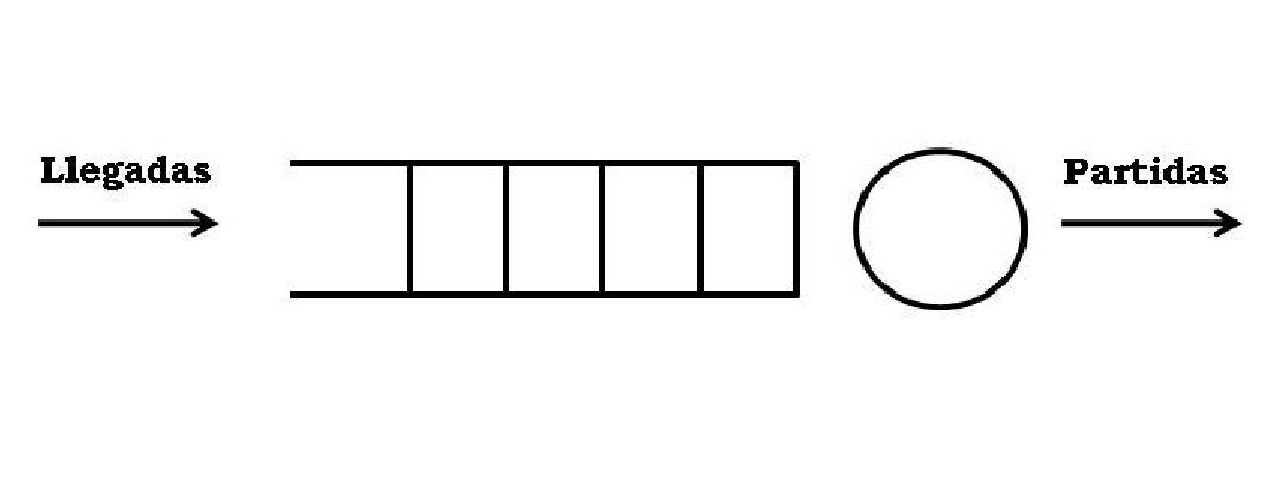
\includegraphics[width=3.2in]{cola2}
\caption{Modelo de cola simple: los clientes llegan por la parte izquierda y entran en el servidor o en la cola, y luego de ser atendidos salen del servidor por la derecha}
\end{center}
\end{figure}

El problema es determinar qu\'e capacidad tiene la cola o qu\'e tasa de servicio tiene el servidor ya
que ni los clientes llegan a tiempos fijos ni los tiempos de servicio son iguales para todos los
clientes. Nosotros utilizamos un modelo de cola simple de tipo M/M/1/$\infty$/FIFO en el que tanto el
tiempo entre arribos de clientes como el tiempo de servicio son variables aleatorias con distribuci\'on
exponencial. Tambi\'en supone que la cola tiene capacidad infinita, y sigue una disciplina de tipo FIFO.\\
En la secci\'on 2 simulamos una cola simple con una simulaci\'on forzada por eventos para obtener una
estimaci\'on de los par\'ametros del sistema. En la secci\'on 3 computamos con un error del 5\% la longitud
promedio de la cola y el tiempo medio de un cliente en la cola, en funci\'on de la intensidad de tr\'afico comparando los
resultados de la simulaci\'on con los valores te\'oricos. En la seccion 4, dise\~namos un modelo
de un sistema de dos colas en serie, y computamos la longitud media de la cola en funci\'on de la intensidad de tr\'afico.
Finalmente en la secci\'on 5, exponemos las conclusiones.

%para meter graficos
%-------------------
%\begin{figure}[t]
%\label{fig:histogramalecuyer}
%\begin{center}
%\centering
%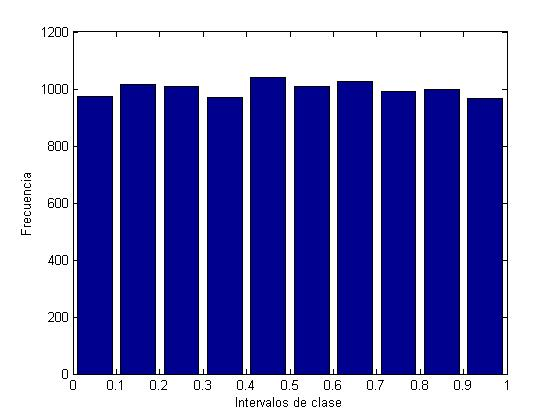
\includegraphics[width=3.2in]{clases.jpg}
%\caption{10000 n\'umeros generados con el generador de L'Ecuyer divididos en 10 intervalos de clase que muestran una distribuci\'on uniforme}
%\end{center}
%\end{figure}

%para meter tablas
%-----------------
%\begin{table}[!t]
%\renewcommand{\arraystretch}{1.3}
%\caption{Semillas de las variables pseudoaleatorias}
%\centering
%\begin{tabular}{c c}
%\hline
%\hline
%Variable  & Semilla\\
%\hline
%$u_1$ &  23\\
%$u_2$ & 2 \\
%$u_3$ & 5 \\
%$u_4$ & 17  \\
%$u_5$ & 7 \\
%\hline
%\hline
%\end{tabular}
%\label{tab:sim}
%\end{table}

%%%%%%%%%%%%%%%%%%%%%%%%%%%%%%%%%%%%%%%%%%%%%%%%%%%%%%%%%%%%%%%%%%%%%%%%%%%%%%%%%%%%%%%%%%%%%%%%%%%%%%%%
\section{Simulando la cola} %seccion 2
%%%%%%%%%%%%%%%%%%%%%%%%%%%%%%%%%%%%%%%%%%%%%%%%%%%%%%%%%%%%%%%%%%%%%%%%%%%%%%%%%%%%%%%%%%%%%%%%%%%%%%%%
El modelo de cola elegido es el m\'as simple de analizar mediante la simulaci\'on forzada por eventos discretos.
La simulaci\'on por eventos discretos es una t\'ecnica inform\'atica de modelado din\'amico de
sistemas. Estos sistemas se caracterizan por mantener un estado interno global que cambia en instantes
de tiempo asociados a la ocurrencia de un determinado evento en la din\'amica del sistema. En nuestro
caso, el conjunto discreto de eventos del sistema es $E=\{llegada, partida\}$, y el conjunto de estados
del servidor es $S=\{libre, ocupado\}$.\\
Para el caso en que el intervalo entre llegadas sea una variable aleatoria exponencialmente distribuida
con tiempo medio entre arribos ($1/\lambda$) de 1 minuto y el tiempo de servicio ($1/\mu$) tambi\'en sea 
exponencial con media de 0.5 minutos; una simulaci\'on forzada por eventos da los resultados de la tabla 1 
(cuando la semilla del generador de n\'umeros aleatorios est\'a seteada en $5$).\\

\begin{table}[!t]
\renewcommand{\arraystretch}{1.3}
\centering
\begin{tabular}{c c}
\hline
\hline
Par\'ametro  				&	Valor			\\
\hline
Tiempo medio en cola		&	0.895 minutos	\\
Longitud media de la cola	&	0.846			\\
Utilizaci\'on del servidor	&	0.464			\\
Simulaci\'on finalizada a	&	1057.655 minutos\\
\hline
\hline
\end{tabular}
\label{tab:sim}
\caption{Resultados de una simulaci\'on forzada por eventos con $\lambda = 1$ minuto y $\mu \sim \epsilon(0.5 minutos)$ para 1000 clientes}
\end{table}

El estado del servidor en esta simulaci\'on lo mostramos en la figura 2, y en la figura 3 mostramos
la longitud de la cola en funci\'on del tiempo.

\begin{figure}[t]%figura 2
\label{fig:estadoservidor}
\begin{center}
\centering
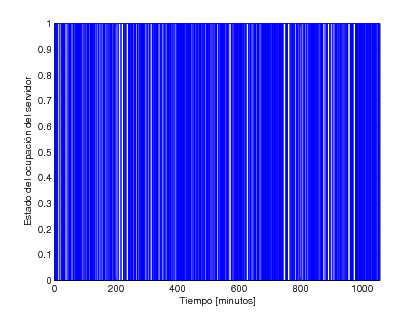
\includegraphics[width=3.2in]{estado_servidor}
\caption{Gr\'afico que muestra el estado del servidor en funci\'on del tiempo. Si el servidor esta desocupado en un instante, el valor es $0$, en caso contrario, el valor es 1.}
\end{center}
\end{figure}

\begin{figure}[t]%figura 3
\label{fig:longitudcola}
\begin{center}
\centering
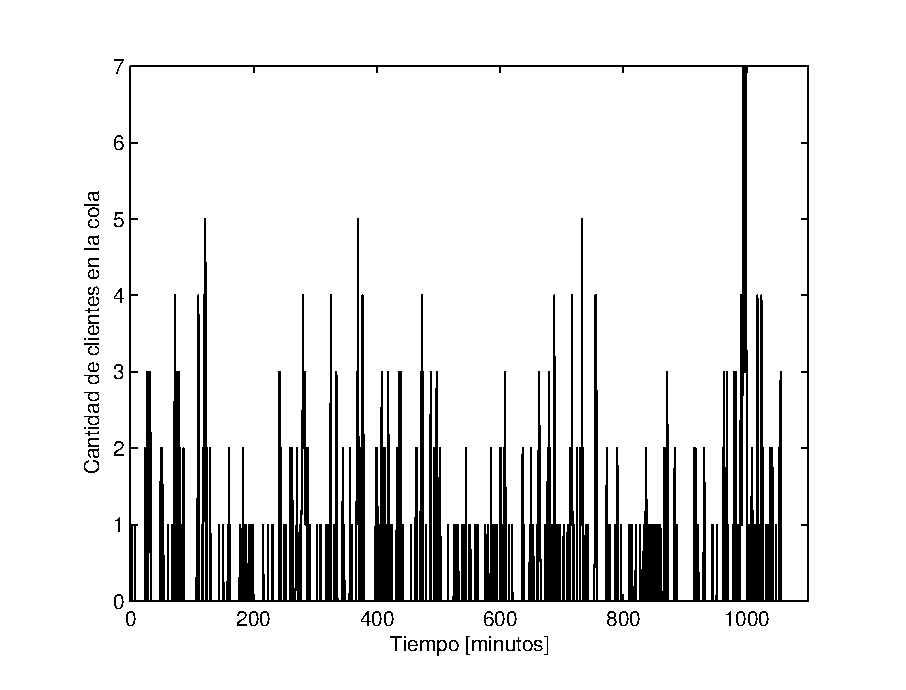
\includegraphics[width=3.2in]{gente_en_cola}
\caption{Gr\'afico que muestra la longitud de la cola en funci\'on del tiempo para la simulaci\'on realizada.}
\end{center}
\end{figure}

Podemos ver en las figuras 2 y 3 que el servidor se encuentra ocupado en casi todo el tiempo, y la cola
llega a un m\'aximo de $7$ sobre el final de la simulaci\'on.

%%%%%%%%%%%%%%%%%%%%%%%%%%%%%%%%%%%%%%%%%%%%%%%%%%%%%%%%%%%%%%%%%%%%%%%%%%%%%%%%%%%%%%%%%%%%%%%%%%%%%%%%
\section{C\'alculo de par\'ametros del sistema} %seccion 3
%%%%%%%%%%%%%%%%%%%%%%%%%%%%%%%%%%%%%%%%%%%%%%%%%%%%%%%%%%%%%%%%%%%%%%%%%%%%%%%%%%%%%%%%%%%%%%%%%%%%%%%%
Para distintos sistemas como podr\'ia ser la cola de un banco, o de cualquier servicio que pueda ser
simulado por el sistema de colas, puede llegar a ser muy \'util conocer distintos par\'ametros como
por ejemplo el promedio temporal de clientes en el sistema, o el tiempo medio que un cliente tarda
en el sistema.

%%%%%%%%%%%%%%%%%%%%%%%%%%%%%%%%%%%%%%%%%%%%%%%%%%%%%%%%%%%%%%%%%%%%%
\subsection{Promedio temporal de clientes en el sistema} %seccion 3.1
%%%%%%%%%%%%%%%%%%%%%%%%%%%%%%%%%%%%%%%%%%%%%%%%%%%%%%%%%%%%%%%%%%%%%
%%%%%%%%%%%%%%%%%%%%<chamuyo>
En un caso pr\'actico, conocer este par\'ametro puede resultar \'util para saber si es necesario
tener otra caja de atenci\'on al cliente, si la cantidad de clientes en el sistema con una sola es demasiado grande.\\
%%%%%%%%%%%%%%%%%%%%<\chamuyo>
Estimamos con un error menor al 5\%, el promedio temporal de clientes en el sistema (L), 
cuyo valor te\'orico se calcula con la ecuaci\'on 1

\begin{equation}
L = \frac{\rho}{1-\rho}
\end{equation}

donde $\rho=\lambda/\mu$ es la intensidad de tr\'afico de la cola.\\
Para lograrlo, simulamos la cola mediante una simulaci\'on forzada por eventos realizada en Matlab.
%%%%%%%%y determinamos que se deben realizar XXXXXXXXXXXXXXXXXXX simulaciones para tener un error menor al 5\%.
Los resultados de la simulaci\'on se ven en la figura 4.

\begin{figure}[t]%figura 4
\label{fig:puntouno}
\begin{center}
\centering
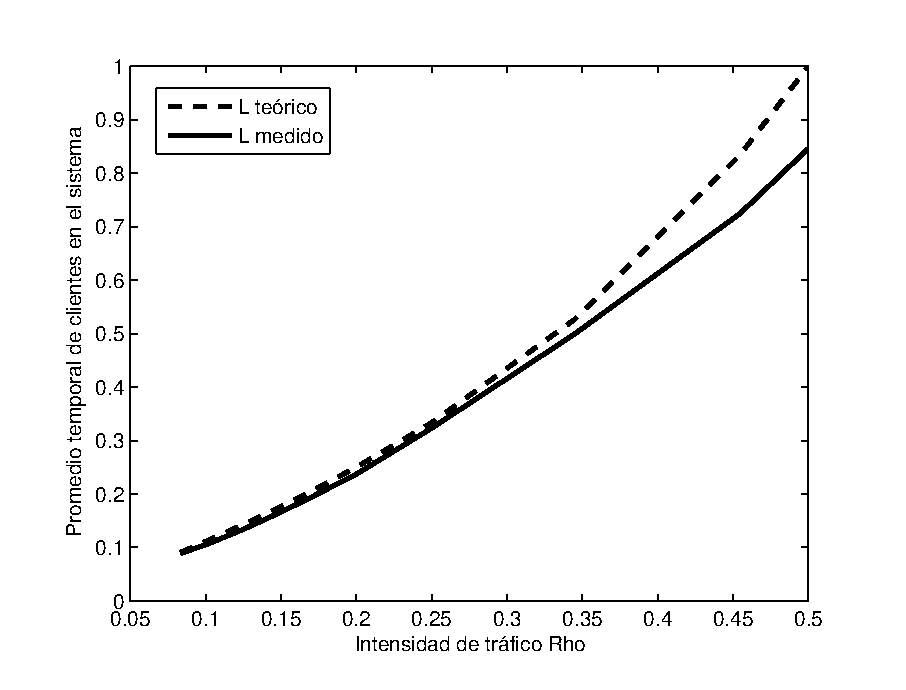
\includegraphics[width=3.2in]{L_rho}
\caption{Promedio temporal de clientes en funci\'on del tr\'afico en el sistema. A medida que el tr\'afico se incrementa, el promedio te\'orico aumenta m\'as r\'apidamente que el valor medido en la simulaci\'on.}
\end{center}
\end{figure}

%%%%%%%%%%%%%%%%%%%%%%%%%%%%%%%%%%%%%%%%%%%%%%%%%%%%%%%%%%%%%%%%%%
\subsection{Tiempo medio de un cliente en el sistema} %seccion 3.2
%%%%%%%%%%%%%%%%%%%%%%%%%%%%%%%%%%%%%%%%%%%%%%%%%%%%%%%%%%%%%%%%%%
En algunos casos, podemos necesitar conocer el tiempo medio que un cliente tarda en el sistema desde
que llega a la cola hasta que sale, luego de ser atendido. \\
El valor te\'orico de este par\'ametro se calcula seg\'un la ecuaci\'on 2

\begin{equation}
  W = \frac{1}{\mu - \lambda}
\end{equation}

donde $\lambda$ es la tasa media de clientes que llegan al sistema (en clientes por minuto) y
$\frac{1}{\mu}$ es el tiempo que tarda el servidor en atender a un cliente.\\
Estimamos este tiempo simulando la misma cola que en la secci\'on 3.1 tambi\'en con un error menor al 5\%.
Los resultados los mostramos en la figura 5.

\begin{figure}[t]%figura 5
\label{fig:puntoccc}
\begin{center}
\centering
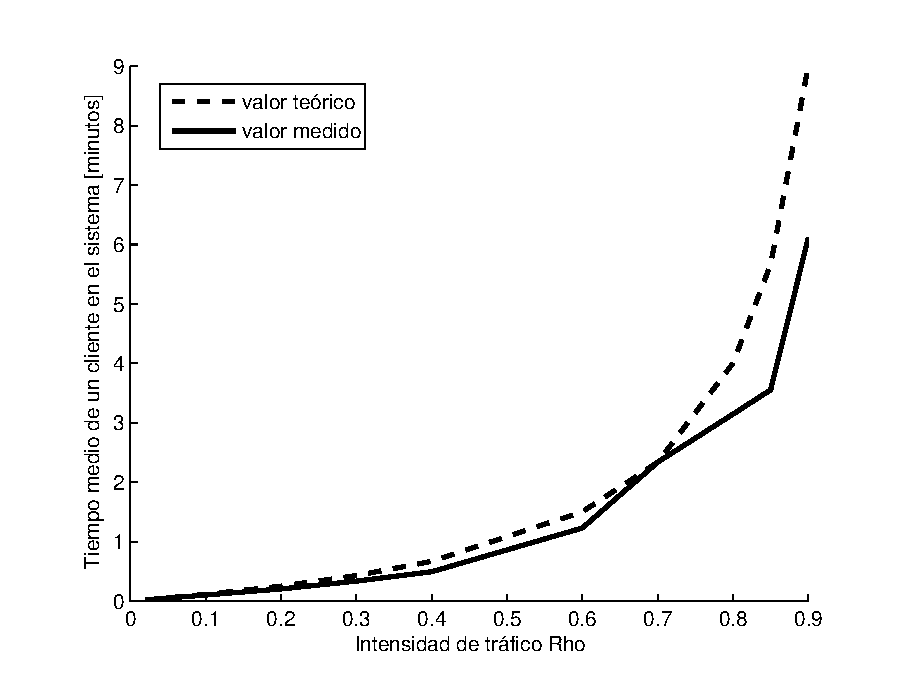
\includegraphics[width=3.2in]{plot_w}
\caption{Gr\'afico del promedio de tiempo en cola por cliente en funci\'on de la intensidad de tr\'afico en el sistema. Podemos observar que a medida que el tr\'afico aumenta, la diferencia entre el valor te\'orico y el de la simulaci\'on aumenta.}
\end{center}
\end{figure}

%%%%%%%%%%%%%%%%%%%%%%%%%%%%%%%%%%%%%%%%%%%%%%%%%%%%%%%%%%%%%%%%%%%%%%%%%%%%%%%%%%%%%%%%%%%%%%%%%%%%%%%%
\section{Sistema de dos colas en serie} %seccion 4
%%%%%%%%%%%%%%%%%%%%%%%%%%%%%%%%%%%%%%%%%%%%%%%%%%%%%%%%%%%%%%%%%%%%%%%%%%%%%%%%%%%%%%%%%%%%%%%%%%%%%%%%
Dise\~namos un sistema m\'as complejo que el de las secciones 2 y 3, haciendo que haya otra cola en serie. 
Cuando un cliente termina de ser atendido en el primer servidor, arriba a la siguiente cola
que se comporta de la misma forma que la cola de las secciones 2 y 3.
Cuando el modelo de colas, representa una cola a continuaci\'on de otra, entonces $\rho$ se calcula como
$\rho = \lambda/(\mu_1+\mu_2)$, siendo $\mu_1$ el tiempo medio de atenci\'on del primer servidor, y 
$\mu_2$ el tiempo de atenci\'on del segundo servidor.
En este caso, simulamos el comportamiento para distintas intensidades de tr\'afico, calculamos
la cantidad media de clientes en el sistema y colocamos los resultados en el gr\'afico de la figura
6.

\begin{figure}[t]%figura 6
\label{fig:puntodos}
\begin{center}
\centering
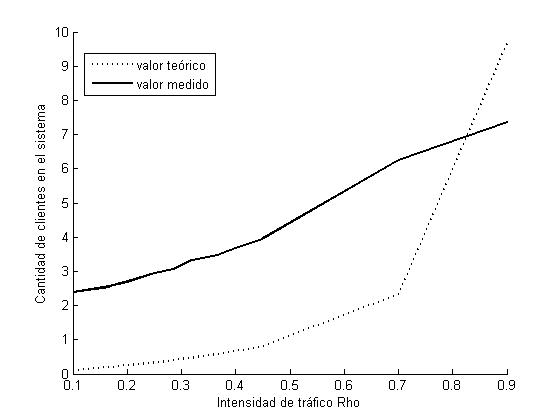
\includegraphics[width=3.2in]{plot_L}
\caption{Gr\'afico de la simulaci\'on del sistema de dos colas en serie. Los valores te\'oricos en este caso no son cercanos a los medidos en la simulaci\'on.}
\end{center}
\end{figure}


%%%%%%%%%%%%%%%%%%%%%%%%%%%%%%%%%%%%%%%%%%%%%%%%%%%%%%%%%%%%%%%%%%%%%%%%%%%%%%%%%%%%%%%%%%%%%%%%%%%%%%%%
\section{Conclusi\'on} %seccion 5
%%%%%%%%%%%%%%%%%%%%%%%%%%%%%%%%%%%%%%%%%%%%%%%%%%%%%%%%%%%%%%%%%%%%%%%%%%%%%%%%%%%%%%%%%%%%%%%%%%%%%%%%
Calculamos los par\'ametros del sistema para un modelo de colas simples, obteniendo como resultado valores
pr\'oximos a los te\'oricos. Sin embargo para un sistema m\'as complejo como el de la secci\'on 4, los
valores medidos no resultaron cercanos a los te\'oricos.
Lo importante de este tipo de simulaciones es obtener estimaciones sobre la cantidad de gente que hay en el sistema,
eso podr\'ia serle \'util a un gerente, para saber el tama\~no que tiene que tener la sala de espera. O incluso,
evaluar el costo de ampliar la sala de espera, contra la posibilidad de contratar otra persona para que atienda a 
los clientes y as\'i reducir el tiempo de espera y la cantidad de personas. 

\begin{thebibliography}{1}

\bibitem{IEEEhowto:kopka}
Teor\'ia de colas, http://exa.unne.edu.ar/depar/areas/informatica/ evalua/teoria\_de\_colas.pdf

\bibitem{IEEEhowto:kopka}
Simulaci\'on de eventos discretos, http://es.wikipedia.org/wiki/Sim ulaci\%C3\%B3n\_por\_eventos\_discretos

\bibitem{IEEEhowto:kopka}
Diaz, Alejandro: Notas de Clase Curso 2009, Simulaci\'on por Eventos Discretos


\end{thebibliography}

\end{document}


